\documentclass{acm_proc_article-sp}

\usepackage{epstopdf}
\usepackage{auto-pst-pdf}
\usepackage{graphicx}
\usepackage[labelfont=bf]{caption}
\usepackage{array}
\usepackage{algorithm}
\usepackage{algpseudocode}

\graphicspath{ {Includes/} }

\begin{document}

\title{A Farewell to Structural Rigidity}
\subtitle{Midterm Project Report}

\numberofauthors{3}
\author{
% 1st. author
\alignauthor Christopher Ross	
% 2nd. author
\alignauthor Jonathan Brant
% 3rd. author
\alignauthor Zak Roessler
}

\maketitle

\section{Introduction}
Image recognition and classification problems have long captured the interest of computer vision researchers \cite{shapiro2001computer, morris2004computer, sonka2008image}.  The ability to process and accurately identify visual input has a vast array of interesting applications across the field of AI and other scientific disciplines.  Unsurprisingly, however, such an undertaking has proven to be a rather ambitious, with one of the primary obstacles being that of scale \cite{DBLP:journals/corr/RussakovskyDSKSMHKKBBF14}.

Perhaps the most straightforward method of processing images is to consider each pixel as a separate input into an artificial neural network (ANN) classifier, with the image resolution defining the distinct number of pixels.  As image resolution increases, however, the number of classifier inputs will similarly grow exponentially, easily reaching inputs in the millions.  Considering each pixel separately quickly becomes an inefficient approach and necessitates a method for dimensionality reduction.

In order to tackle such large problems, this project proposes the use of an evolved autoencoder. Unlike traditional autoencoders wherein the hidden layers (i.e. compressed feature vectors) are specified apriori, the research presented herein uses HyperNEAT to evolve connective CPPNs which in turn produces autoencoders that are, for all practical purposes, scale invariant and whose hidden structure are decided in a more principled manner.


\section{Background}
The fundamentals of traditional autoencoders are introduced along with the relevant details of the HyperNEAT algorithm.

\subsection{Autoencoders}
Autoencoders are artificial neural networks that perform a non-linear form of principal components analysis (PCA) and attempt to extract the most salient features from the visible (input) layer \cite{bourland1988, baldi2012autoencoders}.  A simple autoencoder has a separate input/output pair for each "visible" feature of a domain as well as a fully connected hidden layer that learns the most salient features of the uncompressed features in the visible layer.  More generally, input is being encoded into a compressed representation and subsequently reconstructed.  Figure \ref{figure:exampleautoencoder} depicts the structure and encode/decode phase of a simple autoencoder.

After the compressed feature vector outputs have been decoded into the full feature set, a reconstruction error is calculated and used to determine the representational efficiency/accuracy of the hidden layer.  The reconstruction error for each visible layer node is fed to a supervised training algorithm, most commonly backpropagation, which updates the weights of the autoencoder in a direction that minimizes reconstruction error \cite{stanfordimage}.

\begin{figure}[h]
	\caption{An autoencoder with 6 visible units and 3 hidden units.  The input is encoded from Layer L1 to Layer L2, and decoded from Layer L2 to Layer L3 \cite{stanfordimage}.}
	\centering
	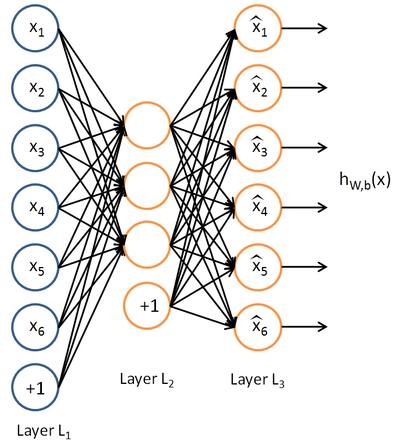
\includegraphics[scale=0.8]{ExampleAutoencoder}
	\label{figure:exampleautoencoder}
\end{figure}

\subsection{NEAT}
In order to automatically determine the autoencoder's hidden layer topology, techniques are borrowed from the field of neuroevolution.  One of the most successful and widely-used genetic algorithms for ANN evolution is the NeuroEvolution of Augmenting Topologies (NEAT).  Three primary components separated NEAT from algorithms that preceded it: growth from minimal structure, speciation, and perhaps most importantly, historical markings \cite{Stanley:2002:ENN:638553.638554}.

Prior to NEAT, many Topology and Weight Evolving Artificial Neural Networks (TWEANNs) began evolution in an already high-dimensional state, leading to slow computationally intensive evolution and often poor results.  NEAT addresses this issue by starting with minimal structure (no hidden nodes) and complexifying only when doing so positively impacts objective performance.  

A potential problem with starting minimally, however, is that such structure will be optimized over time, often out-performing new structural innovations that haven't yet had a chance to be fine-tuned.  NEAT's speciation component avoids premature penalization of new innovations by imposing explicit fitness sharing.  This allows an "adjusted fitness" to be calculated for each genome relative to other structurally similar genomes in its species, thus avoiding premature convergence and protecting new innovations.

Finally, at the core of NEAT are historical markings that uniquely identify each structural innovation.  Historical markings solve the topology matching problem, allowing crossover operations without expensive topological analysis.  Speciation also uses historical markings to determine the species in which to place each genome.

NEAT has been proven to be a highly successful algorithm for control and sequential decision tasks in relatively low-dimensional domains; however, as a direct encoding, the NEAT genotype contains a separate gene for each structural component.  For high-dimensional domains, this can quickly become unwieldy and difficult to optimize.  Moreover, as NEAT considers every input separately, it has no concept of geometric regularities making it a less than optimal choice for domains with a strong visual component.

\subsection{HyperNEAT}
Given the complexity of the domain under consideration and the strong geometric component, the Hypercube-based NeuroEvolution of Augmenting Topologies (HyperNEAT) is a natural choice of algorithms \cite{Stanley:2009:HEE:1516090.1516093}.

As an indirect encoding, HyperNEAT does not impose a one-to-one mapping between genes in the genotype and structural components (i.e. connections and neurons in the case of ANNs) in the phenotype. Instead, HyperNEAT evolves Compositional Pattern Producing Networks (CPPNs) that describe connectivity patterns as a composition of canonical functions \cite{Stanley:2007:CPP:1265496.1265517, Stanley:2009:HEE:1516090.1516093}.  The evolved CPPN queries every possible connection within a 2n-dimensional substrate and outputs the weight of the connection between those two points, effectively drawing an n-dimensional connectivity pattern which is then interpreted as an ANN and evaluated in the given domain.

\begin{figure}[h]
	\caption{The "state-space sandiwch" substrate - ideal for visual mapping \cite{Stanley:2009:HEE:1516090.1516093}.}
	\centering
	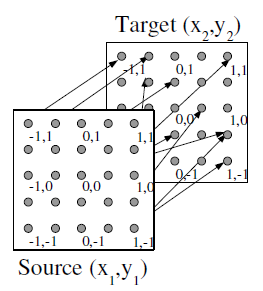
\includegraphics[scale=0.8]{StateSpaceSandwichSubstrate}
	\label{figure:examplesubstrate}
\end{figure}

The substrate configuration is hand-designed in order to accurately represent the geometry of the task-domain.  Among the many possible substrate configurations, one of the most widely used is the "state-space sandwich" substrate wherein a source sheet of neurons is fully connected to a target sheet, as shown in Figure \ref{figure:examplesubstrate}.  A modified version of the state-space sandwich will be used to represent the visible and hidden layers of the desired autoencoder.  HyperNEAT's ability to efficiently generate extremely large scale networks that exhibit virtually no loss of function while using a highly compressed representation that accounts for domain geometry makes it an ideal candidate for the image image processing tasks considered in this paper.

\section{Approach}
While autoencoders have been considered viable methods for data compression or dimensionality reduction since their introduction in 1988 \cite{bourland1988}, they have, to the author's knowledge, always been statically constructed such that their hidden layer is fully specified apriori.  This paper seeks to evaluate the potential of leveraging HyperNEAT for the evolution of autoencoder hidden layer topology.  Results of such an approach will be analyzed both quantitatively (i.e. the efficacy of evolved topology toward reducing reconstruction error) and qualitatively (i.e. how closely does the reconstructed image resemble the original).

The substrate configuration should be chosen to match that of a typical autoencoder structure in order to capture the encode/decode concept.  This includes a two-dimensional sheet of neurons representing each pixel in the given image, a hidden layer sheet with fewer (typically half) neurons, which will in turn be connected to a sheet the same size as the input sheet.  The "hidden layer" sheet effectively represents the hidden layer of a traditional autoencoder.  This "stacked" state-space sandwich is depicted in figure \ref{figure:autoencodersubstrate}.

\begin{figure}[h]
	\caption{The "state-space sandwich" substrate used in the evolved autoencoder experiments.  The hidden layer may vary depending on the experiment configuration, but the general three-tiered structure will remain.}
	\centering
	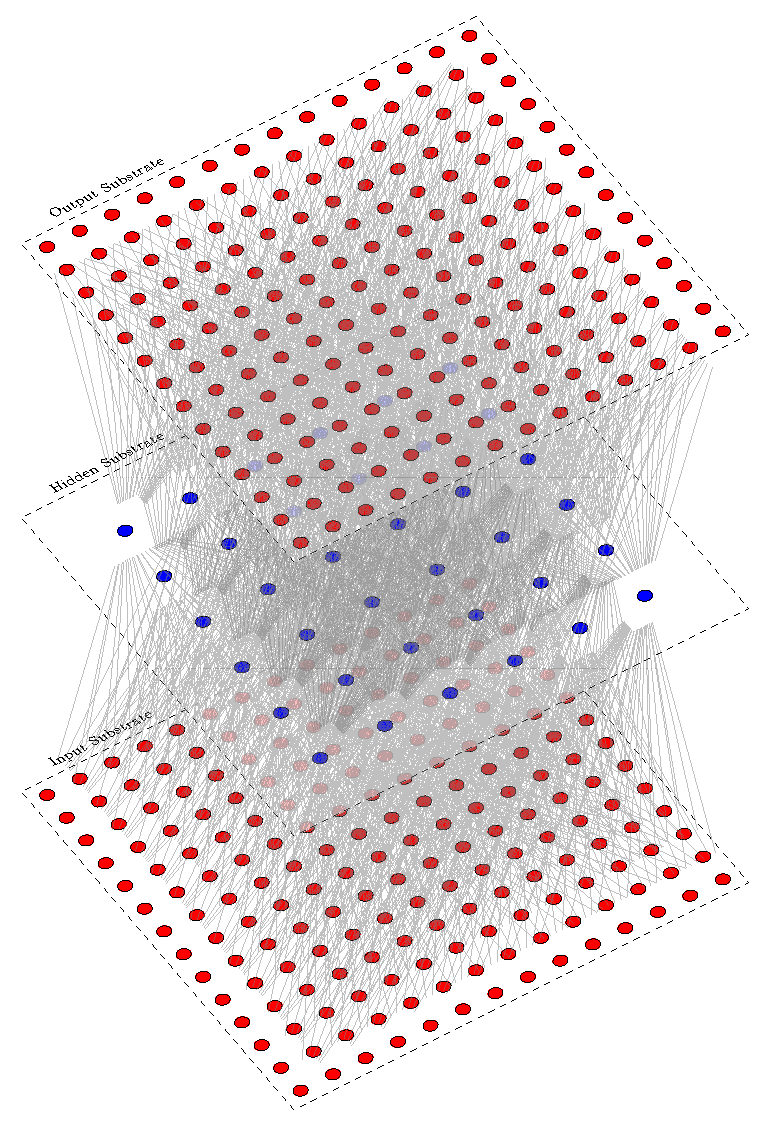
\includegraphics[scale=0.55]{SubstrateConfiguration/AutoencoderSubstrate}
	\label{figure:autoencodersubstrate}
\end{figure}

A HyperNEAT-evolved CPPN will query each possible connection between the input sheet and the hidden sheet as well as between the hidden sheet and the output sheet, outputting the weight for that connection (assuming the weight is of high enough magnitude for the connection to be expressed).  Evolution will begin with a minimally connected CPPN (no hidden nodes) with five input nodes and four output nodes.  The input nodes accept the Cartesian coordinates (x and y position values) for each line segment endpoint and a bias, while the output nodes express the connection weight for the line segment and the bias between the input sheet and the hidden sheet, as well as the same between the hidden sheet and the output sheet.  One such minimal CPPN is shown in figure 4.

The resulting connectivity pattern will be interpreted as an autoencoder and will be both trained and evaluated on samples from the Mixed National Institute of Standards and Technology (MNIST) handwritten digit dataset \cite{mnistdataset}, which is often used as a benchmark dataset for image classification problems.  The handwritten digits in the MNIST dataset are greyscale and each pixel is encoded as an integer in the range 0 to 255 (which represents the intensity of the greyscale pixel).  Reconstruction error for each sample image will be computed based on the difference between the output pixel greyscale intensity compared to its respective input pixel intensity. 

\begin{figure}[h]
	\caption{The minimal, starting-state (no hidden nodes) CPPN.  The inputs to the CPPN are the X and Y coordinates on the source substrate and the X and Y coordinates on the target substrate.  Depending on which layer the CPPN is querying, it will either output the weight of the connection between the input substrate and hidden substrate along with the weight of the bias connection between the same, or the weight of the connection between the hidden substrate and output substrate along with the weight of the bias connection between the same.}
	\centering
	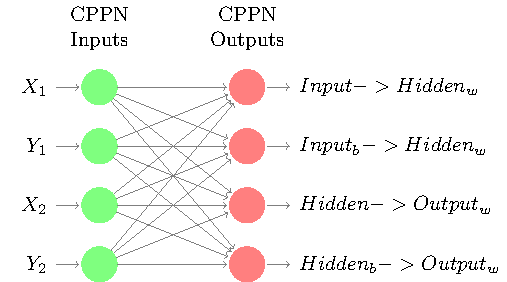
\includegraphics[scale=0.8]{MinimalCppn/MinimalCppn}
	\label{figure:autoencodercppn}
\end{figure}

The training process will use traditional backpropagation (though over arbitrary hidden layer topologies), modifying the autoencoder weights in order to reduce reconstruction error.  After backpropagation has been run for the specified number of iterations (which will vary based on the experiment configuration), the overall reconstruction error will be taken as the score of the CPPN that generated the autoencoder under evaluation.  The maximum fitness attainable is equivalent to the product of the number of validation samples and their resolution (i.e. setting the correct greyscale intensity for each pixel in every validation sample).  Therefore, the fitness score for a given autoencoder evaluation is calculated by subtracting the sum of the reconstruction errors for all validation samples from the maximum fitness, and then dividing by the maximum fitness.  Algorithm 1 describes the full process.

\begin{algorithm*}
	\caption{Autoencoder Training/Evaluation Algorithm}
	\begin{algorithmic}[1]
		\Procedure{EvaluateAutoencoder}{$s,res$} \Comment{Scores autoencoders on $s$ image samples at $res$ resolution}
			\State $max\_fitness \gets s * res$ \Comment {Maximum fitness is product of \# of image samples and their resolution}
			\For{\texttt{Each genome in population}}
				\For{\texttt{Each training image}}
					\While{$iter<n$}\Comment{Backpropagate for $n$ iterations}
						\State \texttt{Activate network}
						\State \texttt{Compute error and update weights}
					\EndWhile
				\EndFor
				\State $error\_sum\gets 0$ \Comment {Initialize the sum of errors}
				\For{\texttt{Each validation image}}
					\For{\texttt{Image pixel}}
						\State $error\_sum := error\_sum + abs(input\_value - output\_value)$ \Comment {Error is magnitude of difference between input and output pixel intensity}
					\EndFor
					\State \texttt{Compute network error in one activation (no backpropagation)}
				\EndFor
				\State $fitness := error\_sum + (max\_fitness - error\_sum) / max\_fitness * 100$
      		\EndFor
   		\EndProcedure
	\end{algorithmic}
\end{algorithm*}

In this way, HyperNEAT is generating the autoencoder starting state and backpropagation is fine tuning it.  The hope is that HyperNEAT will generate a structure that is easily trained to a point of minimal reconstruction error.

\section{Discussion of Current State}
The current state discussion includes the results observed thus far from initial experimentation, an analysis of those results (including alternate strategies in the event that experiment outcomes were poor), and final experiments that are planned to bring the project to a hopefully informative completion.

Recall that results will be analyzed from both a quantitative and qualitative standpoint.  Quantitative analysis is concerned with the final reconstruction error of the networks after evolution and backpropagation while the qualitative analysis is based on a subjective assessment of how closely the reconstructed image matches the original.  Table 1 enumerates the experiment parameters used in both the NEAT and HyperNEAT experiments presented in this section.

\begin{table}[h]
	\caption{HyperNEAT Qualitative Results}
	\small
	\centering
	\begin{tabular}{>{\centering}m{1.7cm} >{\centering}m{2.1cm} >{\centering}m{1.7cm} >{\centering\arraybackslash}m{1.5cm}}
		\hline\hline
		\textbf{Source} & \textbf{Reconstructed} & \textbf{Set} & \textbf{Index} \\
		\hline
		\includegraphics[scale=0.5]{One_Source_Training_Index30} & \includegraphics[scale=0.5]{One_Reconstructed_Training_Index30} & Training & 30 \\
		\includegraphics[scale=0.5]{One_Source_Training_Index60} & \includegraphics[scale=0.5]{One_Reconstructed_Training_Index60} & Training & 60 \\
		\includegraphics[scale=0.5]{One_Source_Validation_Index85} & \includegraphics[scale=0.5]{One_Reconstructed_Validation_Index85} & Validation & 85 \\
		\includegraphics[scale=0.5]{One_Source_Validation_Index95} & \includegraphics[scale=0.5]{One_Reconstructed_Validation_Index95} & Validation & 95 \\
	\end{tabular}
	\label{table:imageresults}
\end{table}

The original images were scaled down from 28x28 pixels (greyscale) to 14x14 for training efficiency.  In order to evaluate the qualitative results, both source and reconstructed images were written to bitmap files and scaled to 800\%. 

\begin{table*}[t]
	\caption{Configuration used for Initial NEAT and HyperNEAT experiments}
	\small
	\centering
	\begin{tabular}{|p{5cm}|p{0.8cm}|p{9cm}|}
		\hline\hline
		\textbf{Parameter} & \textbf{Value} & \textbf{Description} \\
		
		\hline
		
		Training Sample Proportion & 80\% & Percentage of sample images used for training \\
		\hline
		Number of Backpropagation Iterations & 1 & Number of backpropagation iterations performed during training \\
		\hline
		Learning Rate & 0.01 & Learning Rate (to control backpropagation convergence speed) \\
		\hline
		Image Resolution Reduction Factor & 2 & Reduction factor of source image (i.e. a 28x28 image becomes 14x14 with a reduction factor of 2) \\
		\hline
		MNIST Digit & 0, 1 & MNIST handwritten digit dataset image used \\
		
		\hline
	\end{tabular}
	\label{table:initialconfiguration}
\end{table*}

\subsection{NEAT Results}
During the initial stages of experimentation, standard NEAT was used to directly evolve autoencoders.  The result was slow evolution (due to the massive search space) and qualitatively poor image reconstruction.  Figure \ref{figure:neatstartingnetwork} depicts the starting state of a NEAT-evolved autoencoder, with inputs fully connected to a single hidden node, and that hidden node fully connected to the output nodes.  It's state after 1,000 generations is shown in figure \ref{figure:neatevolvednetwork}, with the non-linearities introduced by the additional hidden layer structure aiding in the reduction of training error (though not in the manner hoped for, as described below).

\begin{figure}[h]
	\caption{The starting state of a NEAT-evolved autoencoder.}
	\centering
	\includegraphics[scale=0.17]{NeatStartingState}
	\label{figure:neatstartingnetwork}
\end{figure}

\begin{figure}[h]
	\caption{A NEAT-evolved autoencoder after 1,000 generations of evolution.  Structure has been added in order to aid in reducing training error, but the qualitative results were not quite as expected, resulting in mostly black images.}
	\centering
	\includegraphics[scale=0.17]{NeatEvolvedState}
	\label{figure:neatevolvednetwork}
\end{figure}

Interestingly, while reconstruction error reached about 90\% accuracy form a quantitative standpoint, the qualitative result was a completely black image.  Intuitively, this was because most of the image was just empty, black space and the digit itself occupied a comparatively small number of pixels.

However, the deeper problems was that NEAT was unable to generate a viable autoencoder starting state due to its inability to account for task geometry.  It was primarily this realization that led to the incorporation of HyperNEAT.

\subsection{HyperNEAT Results}

After the fairly underwhelming results with NEAT, HyperNEAT was incorporated in the hopes that incorporating information about the domain geometry would boost qualitative performance.  Figure \ref{figure:autoencodercppn} depicts a fully connected, minimal CPPN (i.e. no hidden nodes) of the form that was used in the below experiments; however, most runs started with a CPPN that was 5\% and connections added as they were found beneficial with regard to reducing training error.  

Figure \ref{figure:minimallyconnectedcppn} depicts such a CPPN, which was evolved in 136 generations and had a fitness of 0.937 (93.7\% accuracy).  Note that the trial that produced this CPPN ran for 136 generations, but it exhibited a very steep increase in fitness in just the first couple of generations as shown in figure \ref{figure:fitnessovergenerations}.  This may be due to the fine-tuning of backpropagation and the highly specific manner in which it rewards networks that are more easily tunable; however, more experimentation is needed in order to determine whether such an assertion is merited.

\begin{figure}[h]
	\caption{A CPPN evolved in 136 generations with a fitness of 0.937 (i.e. 93.7\% reconstruction accuracy).}
	\centering
	\includegraphics[scale=0.3]{MinimallyConnectedCPPN}
	\label{figure:minimallyconnectedcppn}
\end{figure}

\begin{figure}[h]
	\caption{Fitness of an evolved CPPN over 136 generations.  Notice the sharp increase with the first couple of generations followed by relatively stable dynamics.}
	\centering
	\includegraphics[scale=0.17]{FitnessOverGenerations}
	\label{figure:fitnessovergenerations}
\end{figure}

Interestingly, quantitative results for HyperNEAT were quite similar to that of traditional NEAT, with networks consistently training to about 90\% accuracy (given the experiment configuration shown in table \ref{table:initialconfiguration}). However, the manner in which those scores were reached differed considerably.  While NEAT reached such an error by simply turning all pixels black, HyperNEAT managed to produce results that were qualitatively similar to the original.  The figures in table \ref{table:imageresults} depict a sample of the source image and reconstructed images, giving a sense of the autoencoders' qualitative performance.

\subsection{Plan for Completion}

The initial experiments consisted only of two digits from the MNIST dataset using a similarly limited parameter set.  Future experiments will include the following:

\begin{description}
	\item[Training/Validation Proportion:] The proportion of the image sample set used for training versus validation will be varied in order to get an idea of the minimum training sample size required in order to produce acceptance results.
	\item[Maximum Backpropagation Iterations:] The number of iterations of backpropagation that is run will be both increased and decreased in order to determine the right balance between evolution of the autoencoder starting state and the extent to which it needs to be trained following evolution.  Perhaps the most interesting question here is whether evolution can produce robust autoencoders with minimal intervention from gradient-based optimization.
	\item[Image scaling:] Currently, experiments are being run with images that are half the resolution of the original.  These images will be increased to full resolution (28x28 pixels) in order to confirm the ability of HyperNEAT-evolved autoencoders to scale.
	\item[MNIST Generalization:] The experiments run thus far have been limited to the first two digits of the MNIST dataset.  Higher order digits vary significantly in geometric structure and will be a good indication of the evolved autoencoder's ability to reconstruct a wider range of shapes.
\end{description}

\balancecolumns

\bibliographystyle{ieeetran}
\bibliography{MidtermReport}

\end{document}
